
%
%%% Preamble
\documentclass[paper=a4, fontsize=11pt]{scrartcl}	% Article class of KOMA-script with 11pt font and a4 format

\usepackage[french]{babel}
\usepackage[protrusion=true,expansion=true]{microtype}				% Better typography
%\usepackage{amsmath,amsfonts,amsthm}										% Math packages
\usepackage[pdftex]{graphicx}														% Enable pdflatex
\usepackage{color,transparent}													% If you use color and/or transparency
\usepackage[usenames,dvipsnames]{xcolor}
\usepackage[hang, small,labelfont=bf,up,textfont=it,up]{caption}	% Custom captions under/above floats
\usepackage{epstopdf}																	% Converts .eps to .pdf
\usepackage{subfig}																		% Subfigures
\usepackage{booktabs}																	% Nicer tables
\usepackage{listings}

\usepackage{caption}

%%% Advanced verbatim environment
\usepackage{verbatim}
\usepackage{fancyvrb}
\DefineShortVerb{\|}								% delimiter to display inline verbatim text


%%% Custom sectioning (sectsty package)
\usepackage{sectsty}								% Custom sectioning (see below)
\allsectionsfont{%									% Change font of al section commands
	\usefont{OT1}{bch}{b}{n}%					% bch-b-n: CharterBT-Bold font
%	\hspace{15pt}%									% Uncomment for indentation
}

\sectionfont{%										% Change font of \section command
	\usefont{OT1}{bch}{b}{n}%					% bch-b-n: CharterBT-Bold font
	\sectionrule{0pt}{0pt}{-5pt}{0.8pt}%	% Horizontal rule below section
	}

%%% Input Characters
\usepackage[utf8]{inputenc}
%%% Custom headers/footers (fancyhdr package)
\usepackage{fancyhdr}
\pagestyle{fancyplain}
\fancyhead{}														% No page header
\fancyfoot[C]{\thepage}										% Pagenumbering at center of footer
\fancyfoot[R]{\small \texttt{NGUYEN Van Tho - IFI - Promotion 17}}	% You can remove/edit this line 
\renewcommand{\headrulewidth}{0pt}				% Remove header underlines
\renewcommand{\footrulewidth}{0pt}				% Remove footer underlines
\setlength{\headheight}{13.6pt}

%\lstdefinestyle{Shell}{delim=[il][\bfseries]{BB}}
 
\lstset{
 	language=C++,
% 	captionpos=b,
 	tabsize=3,
 	frame=lines,
 	keywordstyle=\color{blue},
 	commentstyle=\color{gray},
 	stringstyle=\color{green},
	extendedchars=true,
% 	numbers=left,
 	numberstyle=\tiny,
 	numbersep=5pt,
 	breaklines=true,
 	showstringspaces=false,
 	basicstyle=\footnotesize\ttfamily,
	emph={label}
}
   %\DeclareCaptionFont{blue}{\color{blue}} 
 
%\captionsetup[lstlisting]{singlelinecheck=false, labelfont={blue}, textfont={blue}}
\DeclareCaptionFont{white}{\color{white}}
\DeclareCaptionFormat{listing}{\colorbox{gray}{\parbox{\textwidth}{#1#2#3}}}
\captionsetup[lstlisting]{format=listing,labelfont=white,textfont=white}
%%% Equation and float numbering
%\numberwithin{equation}{section}															% Equationnumbering: section.eq#
%\numberwithin{figure}{section}																% Figurenumbering: section.fig#
%\numberwithin{table}{section}																% Tablenumbering: section.tab#


%%% Title	
\title{ \vspace{-1in} \usefont{OT1}{bch}{b}{n}		
		\Huge \bfseries \strut Traitement d'images\\
		\Large \bfseries \strut Travail pratique 1
}
\author{
		\usefont{OT1}{bch}{m}{n}
        NGUYEN Van Tho
}
%\institute{
%	Promotion 17\\
%	Institut de la Francophonie pour l'Informatique
%}
\date{}

%%% Begin document
\begin{document}
\maketitle
%\tableofcontents
%%%Section 1
\section{Introduction}
Ce TP effectue à calculer le profil d'intensité des pixels d'une ligne d’une image et de modifier du contraste d’une image. Pour la deuxième partie j'ai choisit 3 méthodes: Transformation linéaire par morceaux, transformation non-linéaire exponentielle (gamma correction) et égalisation de l'histogramme.
J'utilise l'outil make pour compiler le programme. Les fonctions de programme sont choisis par les paramètres. Dans quelque cas, le programme ne fonctionne pas bien quand on entre les valeurs inappropriés.

\section{Profil d'intensité des pixels d'une ligne d’une image}
Pour calculer le profil d'intensité des pixels d'une ligne d’une image je lis tous les points de cette ligne et prend ses valeurs d'intensité.
Une nouvelle image (de taille longueur d'image originale x 256) est créée pour afficher le profil. Des lignes est dessinées entre les points pour afficher le profile d'intensité. 
\begin{lstlisting}
    cv::line(profile, p1, p2, cv::Scalar(255, 255, 255));
\end{lstlisting}
L'intensité d'un point dans cette ligne corresponde à un point dans la ligne de l'image originale par cette fonction:
\begin{center}
$I' = 255 - I$
\end{center}
Où I est intensité de point dans l'image originale et I' est l'intensité de point dans la nouvelle image pour afficher le profil.

\begin{lstlisting}
    cv::Point p1 = cv::Point(p, 255 - l1);
\end{lstlisting}

Pour les images en couleur, 3 lignes sont créées pour 3 couleurs différentes.  
\begin{lstlisting}
    //profile for the color blue
    cv::Point p1 = cv::Point(p, b1);
    cv::Point p2 = cv::Point(p + 1, b2);
    cv::line(profile, p1, p2, cv::Scalar(255, 0, 0));
 		...
    //profile for the color red 
    p1 = cv::Point(p, r1);
    p2 = cv::Point(p + 1, r2);
    cv::line(profile, p1, p2, cv::Scalar(0, 0, 255));
\end{lstlisting}

Créer l'image avec une ligne:
\begin{lstlisting}
    cv::Point p1 = cv::Point(0, line);
    cv::Point p2 = cv::Point(imageSize.width - 1, line);
    cv::line(withLine, p1, p2, cv::Scalar(0, 0, 0));
\end{lstlisting}
Quelques expériences avec des images différentes:

Pour créer le profil d'intensité, on lance le programme avec le paramètre: profile un nombre de ligne:
\begin{lstlisting}[label=lancer,caption=commande pour lancer le programme]
 %./tp1 Nom_de_fichier_image profile <ligne>
\end{lstlisting}
Les sorties du programme sont une image de profil et une version modifiée d'image originale (avec une ligne noire horizontale).
Pour montrer le programme. Je le lance avec une image en niveau gris et une image en couleur. 
\subsection{Profil d'intensité des pixels d'une ligne d’une image en niveau gris}
\begin{lstlisting}[label=gris,caption=commande]
 %./tp1 Fig0109-f-organic-superconductor.tif profile 310
\end{lstlisting}
Le résultat est affiché dans l'image ci-dessous. Le programme prend la ligne 310 de l'image. On peut voir dans le profil d'intensité, les valeurs à gauche sont plus grandes que celles à droit car dans l'image originale, les pixels à gauche sont plus clair.
\begin{figure}[h]
	\begin{center}$
		\begin{array}[h]{cc}
		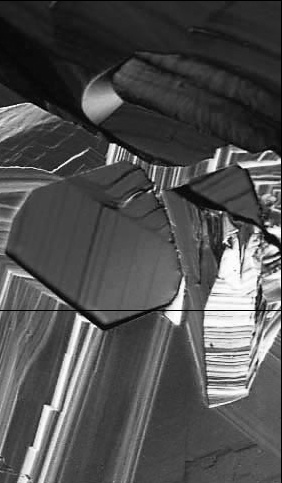
\includegraphics[width=4cm]{images/grayscale.jpg} &
		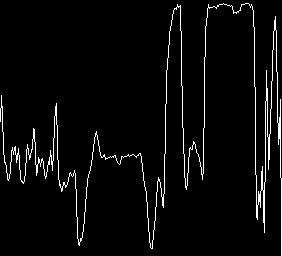
\includegraphics[width=4cm]{images/profilegrayscale.jpg}
		\end{array}$
	\end{center}
	\caption{Profil d'intensité des pixels d'une ligne d’une image en niveau gris}
\end{figure}
\subsection{Profil d'intensité des pixels d'une ligne d’une image en couleur}
\begin{lstlisting}[label=gris,caption=commande]
 %./tp1 piment.jpg profile 400
\end{lstlisting}
Le résultat est affiché dans l'image ci-dessous. Le programme prend la ligne 400 de l'image. On peut voir dans le profil d'intensité, il y a trois lignes en rouge, en vert et en bleu correspondant à intensité de trois couleurs d'image.\\
C'est une image des piments vert et rouge. Nous constatons qu'à coté à gauche de profil, le ligne verte est plus haute et à droit la ligne rouge domine les deux autres couleurs. En effet, coté à gauche d'image contient les piments verts et coté à droit contient les piments rouges. Au centre de profil, nous voyons que les intensités des trois couleurs sont assez grandes car c'est la couleur jaune sombre du bois.  
\begin{figure}[h]
	\begin{center}$
		\begin{array}[h]{cc}
		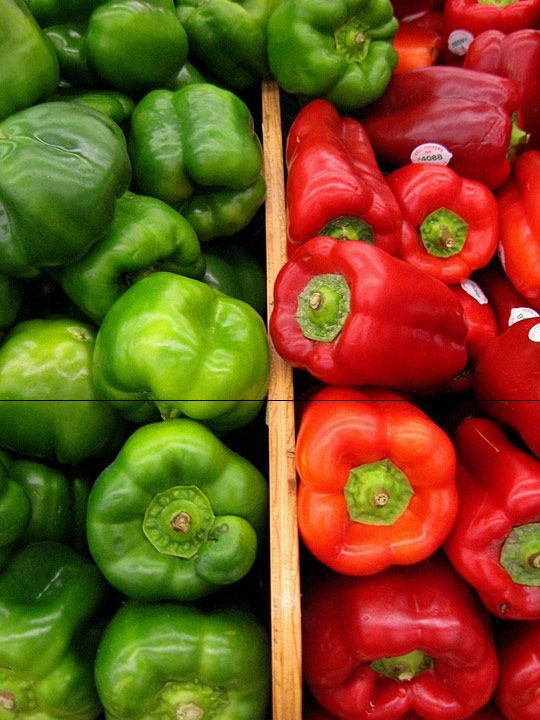
\includegraphics[width=4cm]{images/vn100.jpg} &
		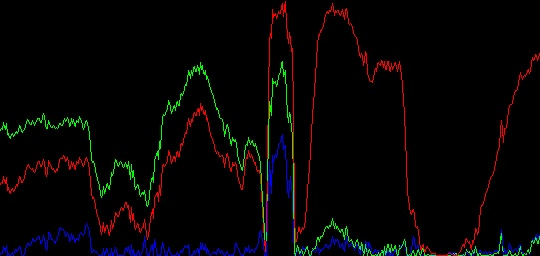
\includegraphics[width=4cm]{images/profilevn100.jpg}
		\end{array}$
	\end{center}
	\caption{Profil d'intensité des pixels d'une ligne d’une image en couleur RGB}
\end{figure}

\section{Modification du contraste d’une image}
\subsection{Linaire avec plusieurs point}
L'objectif de cette méthode est de redistribuer la distribution de l'histogramme d'image. Le contraste est élargi pour avoir le meilleur contraste.
Dans ce TP j'ai implémenté la méthode linaire avec plusieurs morceaux. Les morceaux sont entrés par les paramètres de shell:
\begin{lstlisting}[label=command,caption=commande pour traitement linaire de contraste]
./tp1 nom_de_image linear  x1 y1  x2 y2 .... xn yn
\end{lstlisting}
Le méthode est divisée en trois parties. Première partie est pour traiter le premier morceau.
La nouvelle intensité est calculée par cette formule:
\begin{center}
$I'=y2*(i - x1)/(x2 - x1)$
\end{center}
\begin{lstlisting} [label=premiere,caption=Intensité des points appartenant à premier morceau]
    int v = p2.y*(i - p1.x)/(p2.x - p1.x);
    lut[i] = getIntensity(v, 0, p2.y);
\end{lstlisting}

La deuxième partie est pour traiter les morceaux au milliers. La nouvelle intensité est calculée par cette formule:
\begin{center}
$I'=y1 + (y2 - y1)(i - x1)/(x2 - x1)$
\end{center}
\begin{lstlisting}[label=command,caption=commande pour traitement linaire de contraste]
    int v = p1.y + (p2.y - p1.y)*(i - p1.x)/(p2.x - p1.x);
    lut[i] = getIntensity(v, p1.y, p2.y);
\end{lstlisting}

La troisième partie est pour traiter le dernier morceau. La nouvelle intensité est calculée par cette formule:
\begin{center}
$I'=y1 + (255 - y1)(i - x1)/(x2 - x1)$
\end{center}

\begin{lstlisting}[label=command,caption=commande pour traitement linaire de contraste]
    int v = p1.y + (255 - p1.y)*(i - p1.x)/(p2.x - p1.x);
    lut[i] = getIntensity(v, p1.y, 255); 
\end{lstlisting}
Où getIntensity est la méthode pour normaliser la valeur d'un point p1, p2 sont les points aux bouts des morceaux. qui sont définis par un struct:

\begin{lstlisting}[label=point,caption=la structure point]
struct point{
    uchar x;
    uchar y;
};
\end{lstlisting}
\subsubsection*{Expérimentations et résultats}
Dans cette partie je teste le programme avec deux images. Les résultats sont affichés dans les figure 3 et figure 4.
\begin{lstlisting}
./tp1 militaire.jpg linear 0 0 180 30 200 130 230 220 255 255
./tp1 homme.jpg linear  0 0 70 120 150 200  255 255
\end{lstlisting}
\begin{figure}[htp]
	\begin{center}
		\begin{tabular}[h]{cc}
		\includegraphics[width=4cm]{../militaire.jpg}&
		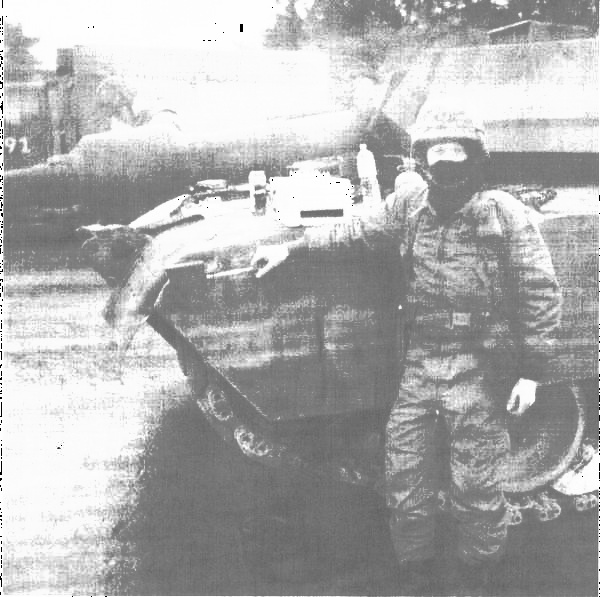
\includegraphics[width=4cm]{images/linearMili.jpg} \\	
		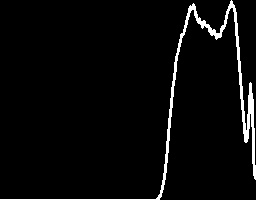
\includegraphics[width=4cm]{images/histMiliAvant.jpg}&
		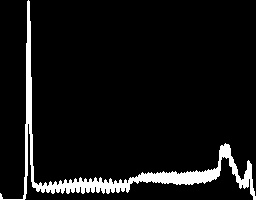
\includegraphics[width=4cm]{images/histMili.jpg}	
		\end{tabular}
			\caption{Un bon exemple de la méthode linaire}
		\begin{tabular}[h]{cc}
		\includegraphics[width=4cm]{../olympic.jpg}&
		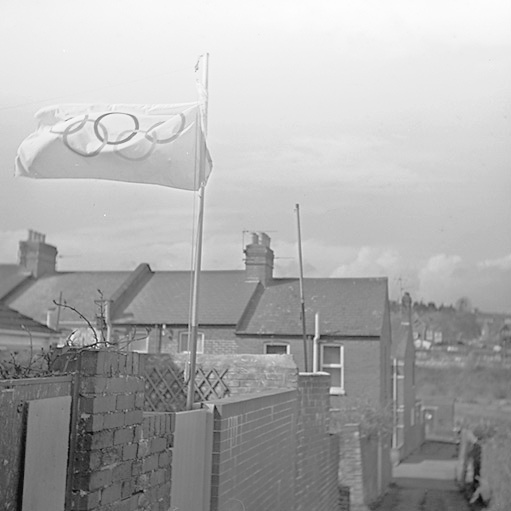
\includegraphics[width=4cm]{images/olym.jpg} \\	
		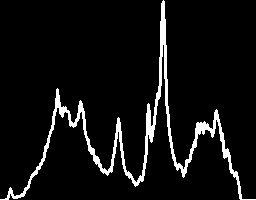
\includegraphics[width=4cm]{images/histolym.jpg}&
		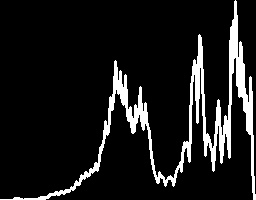
\includegraphics[width=4cm]{images/histolymAvant.jpg}	
		\end{tabular}
	\end{center}
	\caption{Un mauvaise exemple de la méthode linaire}
\end{figure}

Dans le premier cas, le résultat est très bon, le contraste de la nouvelle image est amélioré par rapport au celui de l'image originale. On peut voir dans l'histogramme de la nouvelle image, les pixels sont distribués sur presque tout la domaine de niveau de gris. Au contrait, les pixels sont distribués sur 1/3 dernier du niveau de gris.

Dans le deuxième cas, le résultat n'est pas bon. Le contraste n'est pas amélioré. La nouvelle image a plus de lumière. Cela arrive à cause de la distribution de l'histogramme, il répande de 0 à 255. 

Cette méthode fonctionne bien sur les images dont les histogrammes distribuent dans une partie de niveau de gris. Par exemple, dans la premier cas, il est distribué de 180 à 255. Néanmoins, cette méthode ne fonctionne pas bien sur les image qui contient à la fois des pixels très sombres et des pixels très clairs.
  
\subsection{Non-linaire - correction de gamma}

L'intensité d'un pixel de la nouvelle image est calculé par cette formule:
\begin{center}
$I'=k*255*(I/255.0)^{\gamma}$
\end{center}
\begin{lstlisting}[label=gamma,caption=Implémentation de correction de gamma]
    for (int i = 0; i < 256; i++){                                                     
        float v = 255*pow(i/255.0, gamma);
    }
\end{lstlisting}    
Où k est un coefficient. Dans mon programme, j'ai choisi de fixer cette valeur à 1.
\subsubsection*{Expérimentations et résultats}
Pour montre cette fonction, je teste le programme par cette commande:
\begin{lstlisting}
%./tp1 bicycle.jpg nonlinear 2.2
\end{lstlisting}
Le résultat est affiché dans la figure ci-dessous:
\begin{figure}[h]
	\begin{center}$
		\begin{array}[h]{cc}
		\includegraphics[width=4cm]{../bicycle.jpg}&
		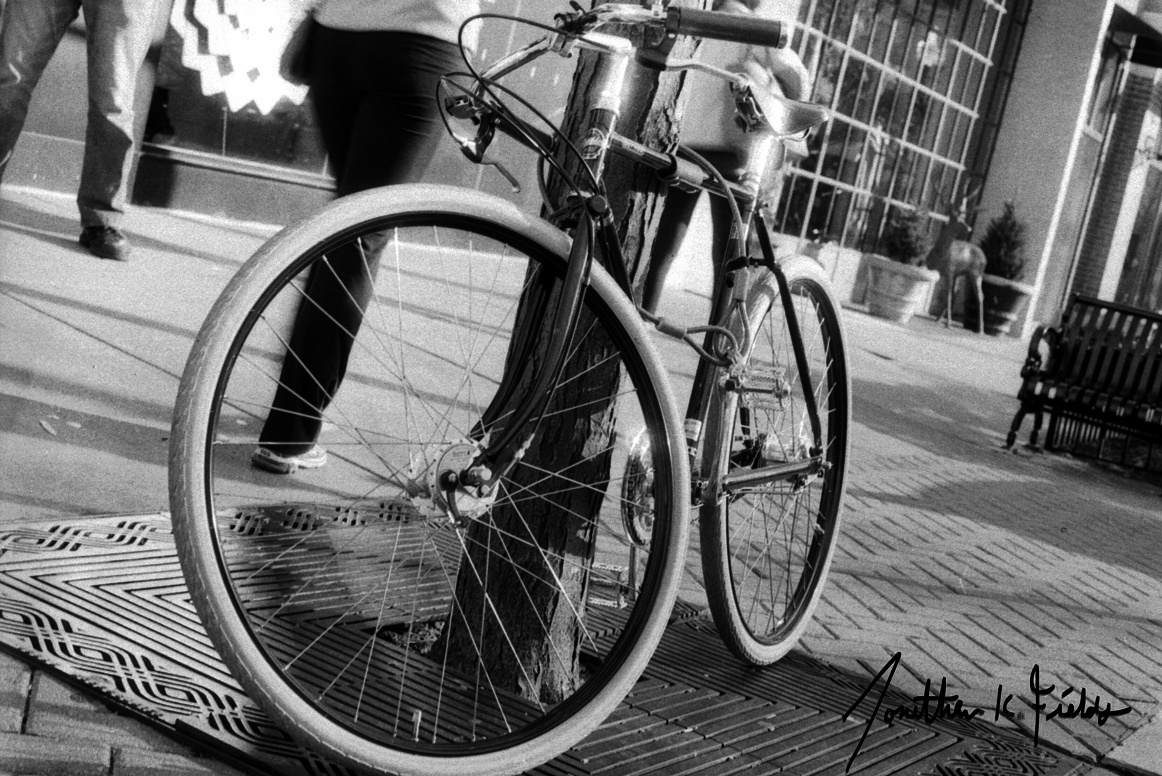
\includegraphics[width=4cm]{images/bicycle-gamma-correction.jpg} \\	
		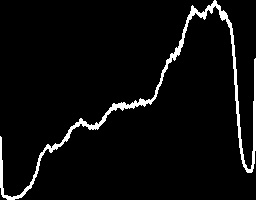
\includegraphics[width=4cm]{images/histbicAvant.jpg}&
		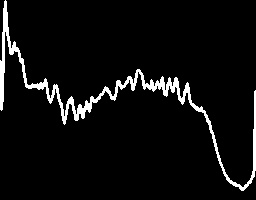
\includegraphics[width=4cm]{images/histbic.jpg}			
		\end{array}$		
	\end{center}
	\caption{La correction de gamma}
\end{figure}

Comparer deux images on constate que l'image après la correction (à droit) est beaucoup meilleur que l'origine. C'est parce que l'origine a la plupart des pixels en grand niveau de gris. La correction gamma avec la valeur appropriée de gamma redistribue l'histogramme de l'image, donc l'image corrigée est meilleur pour les yeux.  

\subsection{Égalisation de l'histogramme}
On essai de redistribue également l'histogramme de l'image, donc améliore le contraste de l'image. L'implémentation d'égalisation de l'histogramme est affichée dans la figure ci-dessous:
\begin{lstlisting}[label=Egalisation,caption=Egalisation de l'histogramme]
    for (int i = 0; i < 256; i++){
        for(int j = 0; j < i; j++){
            c[i] += histNormalised[j];
        }
    }
    for (int i = 0; i < image.size().width; i++){
        for (int j = 0; j < image.size().height; j++){
            imageTransformed.at<uchar>(j, i) = 255*c[image.at<uchar>(j, i)]; 
        }
    } 
\end{lstlisting}
\subsubsection*{Expérimentations et résultats}
Pour montre cette fonction, je teste le programme par cette commande:
\begin{lstlisting}
%./tp1 ./tp1 sat_map4.jpg equalisation
\end{lstlisting}
Le résultat est affiché dans la figure ci-dessous:
\begin{figure}[h]
	\begin{center}$
		\begin{array}[h]{cc}
		\includegraphics[width=4.5cm]{../sat_map4.jpg}&
		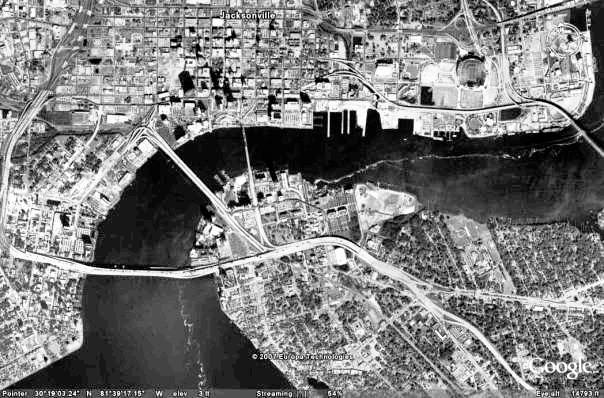
\includegraphics[width=4.5cm]{images/sat.jpg} \\	
		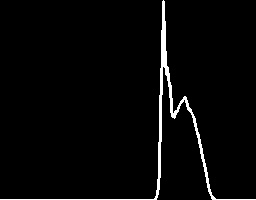
\includegraphics[width=4.5cm]{images/histsatAvant.jpg}&
		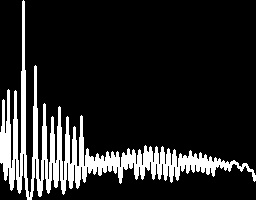
\includegraphics[width=4.5cm]{images/histsat.jpg}			
		\end{array}$		
	\end{center}
	\caption{La correction de gamma}
\end{figure}

On constate que l'image après avoir égalisé (celle à droit) de l'histogramme est beaucoup meilleure que l'origine car l'histogramme est distribué assez égal après avoir appliqué méthode égalisation de l'histogramme. Au contrait, l'image originale a un histogramme distribuant sur un domaine petit. 
\section{Conclusion}
Dans ce TP j'ai implémenté les fonctions pour calculer le profil d'une ligne d'une image, trois méthodes de modifier le contraste d'image: transformation linaire avec morceaux, la correction de gamma et égalisation de l'histogramme. 

La méthode transformation linaire avec morceaux fonctionne bien dans les cas que la distribution de l'histogramme des images ne s'étende pas sur tout le domaine de niveau de gris. En revanche, les images dont les histogrammes étendent sur tout le domaine de gris, cette méthode ne fonctionne pas bien, parfois le résultat peut être moins bon que l'origine. Une autre difficulté de cette méthode est le choix de morceaux, il peut influencer beaucoup la qualité de la transformation. L'image sortie peut avoir des bruits car l'intensité d'un point transformé peut dépasser la valeur maximum de niveau de gris.

La méthode correction de gamma fonctionne bien, notamment dans les cas le gamma ne sont pas correct. Pour avoir le meilleur résultat on doit trouver la valeur optimale de gamma.

La méthode égalisation de l'histogramme fonctionne bien et produit fiable les résultats.

Dans la partie de modifier le contraste, je n'ai pas implémenter pour les images en couleur. Ce la reste comme un travail au futur.
\end{document}